\section{Methodology}

\subsection{Model Architecture}

\subsubsection{ConvNeXt}

ConvNeXt is a modern convolutional neural network (CNN) architecture inspired by Vision Transformers (ViTs). It modernizes standard convolutional operations without relying on self-attention mechanisms. Specifically, ConvNeXt redesigns the standard ResNet architecture by adopting $7 \times 7$ depthwise convolution to enlarge the receptive field, using inverted bottleneck blocks, replacing Batch Normalization with LayerNorm, and replacing Rectified Linear Unit (ReLU) with GELU to improve optimization stability during transfer learning \cite{Liu2022}. These architectural refinements enhance feature representation without sacrificing the computational advantages of convolution-based networks. Fig.~\ref{fig:convnext_block} illustrates the internal structural flow of a ConvNeXt block.

\begin{figure}[htbp]
    \centering
    \resizebox{\columnwidth}{!}{
        \begin{tikzpicture}[
            block/.style={
                rectangle,
                draw=gray!80,
                fill=gray!20,
                minimum width=1.5cm,
                minimum height=2.5cm,
                rounded corners=5pt,
                align=center,
                font=\small\sffamily
            },
            arrow/.style={
                ->,
                >=Stealth,
                thick
            },
            add/.style={
                circle,
                draw,
                minimum size=0.5cm,
                inner sep=0pt
            }
        ]
            \coordinate (input) at (0,0);

            \node [block, right=1cm of input] (b1) {d7$\times$7, 96};
            \node [block, right=1cm of b1] (b2) {1$\times$1, 384};
            \node [block, right=1cm of b2] (b3) {1$\times$1, 96};
            \node [add, right=0.5cm of b3] (plus) {};

            \draw[thick] (plus.north) -- (plus.south);
            \draw[thick] (plus.west) -- (plus.east);

            \coordinate [right=0.5cm of plus] (output);

            \coordinate (split) at (0.5,0);

            \draw [thick] (input) -- (b1.west) node[midway, above, font=\scriptsize\sffamily] {96-d};
            \draw [arrow] (b1.east) -- (b2.west) node[midway, above, font=\scriptsize\sffamily] {LN};
            \draw [arrow] (b2.east) -- (b3.west) node[midway, above, font=\scriptsize\sffamily] {GELU};
            \draw [arrow] (b3.east) -- (plus.west);
            \draw [arrow] (plus.east) -- (output);

            \draw [arrow] (split) -- (0.5,-1.5)
                                -- ([yshift=-1.5cm]plus.center)
                                -- (plus.south);

        \end{tikzpicture}
    }
    \caption{ConvNeXt Block Architecture.}
    \label{fig:convnext_block}
\end{figure}

To evaluate its real-world efficacy, a recent large-scale study compared ConvNeXt, RegNet, and ResNet across $22$ publicly available retinal fundus datasets \cite{Chopowiec2023}. This benchmark comprised more than $125,000$ images spanning normal cases, diabetic retinopathy, glaucoma, and age-related macular degeneration to construct a clinically representative screening model. Among the tested architectures, ConvNeXt-Tiny achieved the best overall performance across most evaluation metrics, obtaining an overall accuracy of $80.46 \pm 1.48\%$. It demonstrated particularly high disease recognition accuracy for glaucoma ($97.20\%$), age-related macular degeneration ($98.14\%$), and diabetic retinopathy ($80.66\%$) These findings demonstrated ConvNeXt-Tiny's reliability for retinal disease classification while maintaining a relatively lightweight architecture, making it highly suitable for transfer learning on moderately sized retinal fundus datasets.

\subsubsection{DeiT}

Standard Vision Transformers (ViTs) rely primarily on self-attention mechanisms to capture long-range dependencies across an entire image and generally require extremely large-scale pretraining datasets to achieve competitive performance \cite{dosovitskiy2021imageworth16x16words}. To overcome these substantial data requirements while preserving the advantages of transformer-based architectures, Data-efficient Image Transformers (DeiT) were proposed \cite{touvron2021trainingdataefficientimagetransformers}.
DeiT introduces a dedicated distillation token into the architecture, which is appended alongside the class token and patch embeddings as illustrated in Fig.~\ref{fig:deit_block}. During training, this token interacts with the patch tokens via self-attention to learn complementary features from a robust, pretrained teacher model (typically a CNN). This mechanism significantly improves classification accuracy, particularly for smaller transformer models, while maintaining computational efficiency.

\begin{figure}
    \centering
    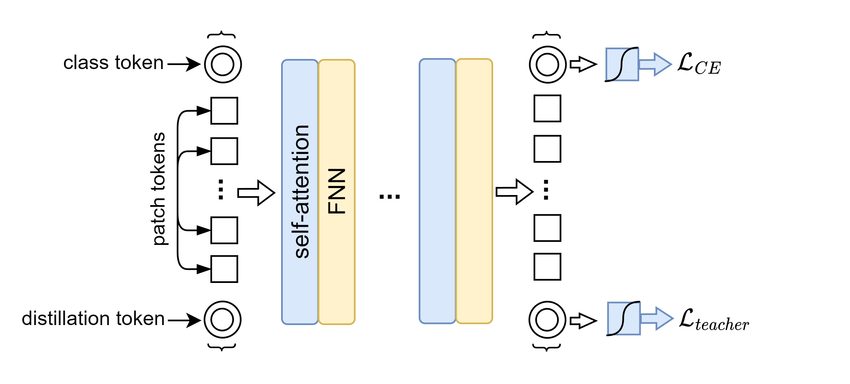
\includegraphics[width=0.45\textwidth]{figures/DeiT-main-architecture.png}
    \caption{DeiT Block Architecture}
    \label{fig:deit_block}
\end{figure}

The data-efficient design of DeiT makes it particularly suitable for medical image analysis, where large annotated datasets are often unavailable and training standard ViTs from scratch is difficult. A recent study incorporated DeiT as one of the transformer-based feature extractors in a hybrid framework for multi-class eye disease classification, demonstrating that combining DeiT with machine learning classifiers contributed to a stacking model that achieved $97.163\%$ classification accuracy on a benchmark retinal dataset \cite{AlMohimeed2025}. These findings indicate that transformer-based models can be effectively applied to retinal disease classification when equipped with efficient training or feature extraction strategies. Therefore, DeiT is suitable for transfer learning as a representative data-efficient Vision Transformer for a moderately sized retinal fundus datasets.

\subsubsection{Hyperparameter \& Model Selection}

Model parameters refer to the network weights that are automatically learned through backpropagation, whereas hyperparameters are predefined before or during training to control the optimization process, regularization, and learning schedule \cite{Bengio2000}. During transfer learning and fine-tuning, commonly configured hyperparameters include the learning rate, batch size, weight decay, optimizer, learning-rate scheduler, data augmentation strategy, number of training epochs, and early stopping criterion. Hyperparameter optimization can be performed using several strategies, including grid search, random search, and manual tuning. Out of those three, random search is generally more efficient than grid search because only a small subset of hyperparameters typically has a significant influence on model performance, and the importance of individual hyperparameters may vary across different datasets \cite{JMLR:v13:bergstra12a}.

To ensure an unbiased evaluation, the dataset is divided into training, validation, and testing subsets. The training set is used to optimize the model parameters, whereas the validation set is exclusively used to select the best hyperparameter configuration and training scenario \cite{Reyes2024}. The test set is used solely for the final performance evaluation and is not involved in any stage of model selection or hyperparameter optimization \cite{Jiang2021}. This separation prevents information leakage and optimistic bias, resulting in a more reliable estimation of the model's generalization capability.

\subsection{Explainable AI (XAI) on Computer Vision}

\subsubsection{Grad-CAM}

For a target class $c$, Grad-CAM first backpropagates the class score $y^c$ with respect to each feature map $A^k$ in the final convolutional layer. The importance weight of the $k$-th feature map is obtained by applying global average pooling to the spatial gradients, which is defined as

\begin{equation}
\alpha_{k}^{c} = \frac{1}{Z} \sum_{i} \sum_{j} \frac{\partial y^{c}}{\partial A_{i,j}^{k}}
\label{eq:grad_cam_weights}
\end{equation}

where $Z$ denotes the total number of spatial locations in the feature map. The resulting weight $\alpha_k^c$ represents the contribution of feature map $A^k$ to the prediction of class $c$ \cite{Selvaraju2020}.

The class activation map is subsequently generated as a weighted combination of all feature maps,

\begin{equation}
    L_{Grad-CAM}^{c} = ReLU (\sum_{k} \alpha_{k}^{c} A^{k})
    \label{eq:grad_cam_activation_map}
\end{equation}

where the ReLU suppresses negative activations, preserving only features that positively influence the prediction of the target class \cite{Selvaraju2020}.

Although originally developed for CNNs, Grad-CAM has been successfully adapted to Vision Transformers. The method utilizes the patch token representations extracted from the final transformer encoder block, which are reshaped into a two-dimensional spatial grid before gradient computation. The spatial gradients are globally averaged to obtain token importance weights, followed by weighted aggregation and ReLU activation to produce the final saliency map \cite{Alhafdhi2026, Vanitha2025}.

Grad-CAM has been widely adopted in medical image analysis to verify whether deep learning models focus on clinically relevant anatomical structures or pathological lesions. As summarized in Table~\ref{tab:medical_gradcam_comparison}, Grad-CAM has demonstrated its effectiveness across multiple imaging modalities and deep learning architectures.

\begin{table}[htbp]
    \caption{Applications of Grad-CAM in Medical Image Analysis.}
    \label{tab:medical_gradcam_comparison}
    \centering
    \small
    \setlength{\tabcolsep}{4pt}
    \begin{tabularx}{\columnwidth}{>{\raggedright\arraybackslash}p{2.6cm} >{\raggedright\arraybackslash}p{2cm} >{\raggedright\arraybackslash}X}
        \toprule
        \textbf{Medical Domain} & \textbf{Architecture} & \textbf{Interpretability Outcome} \\
        \midrule
        Chest X-ray (TB) &
        ViT &
        Highlights diagnostically relevant pulmonary regions, enabling visualization of the model's focus during tuberculosis classification \cite{Vanitha2025}.\\
        \addlinespace

        Retinal disease &
        ResNet101-V2 &
        Emphasizes retinal abnormalities associated with glaucoma, diabetic retinopathy, and cataracts, improving multiclass model interpretability \cite{AbdEl-Ghany2025}.\\
        \addlinespace

        Thyroid ultrasound &
        Hybrid CNN--ViT &
        Produces clinically meaningful activation patterns that validate lesion localization and support prediction reliability \cite{Alhafdhi2026}.\\
        \bottomrule
    \end{tabularx}
\end{table}

\subsubsection{Attention Rollout}

Vision Transformers compute a self-attention matrix at every transformer layer, where each element represents the attention weight assigned from one token to another. Since each image patch is represented as a token, the attention matrix describes how information is exchanged among all image patches through the self-attention mechanism. Self-attention enables every token to interact with all other tokens, allowing the model to capture global contextual relationships, unlike convolutional neural networks that rely on local receptive fields \cite{dosovitskiy2021imageworth16x16words}.

However, the attention matrix from a single transformer layer only reflects the interaction at that particular layer and does not directly indicate the overall contribution of an input patch to the final prediction. To estimate how information propagates throughout the transformer, Attention Rollout recursively composes the attention matrices from consecutive layers. Consequently, the importance of each input patch is determined by the accumulated attention flow from the input layer to the final class token representation \cite{Abnar2020}.

The recursive formulation of Attention Rollout is expressed as

\begin{equation}
    \tilde{A}(l_{i}) = \begin{cases}
        {A}(l_{i}) \tilde{A}(l_{i-1})   & \text{if } i > j\\
        {A}(l_{i})                      & \text{if } i = j
    \end{cases}
    \label{attention_rollout_equation}
\end{equation}

where $A(l_i)$ denotes the attention matrix of the $i$-th transformer layer, while $\tilde{A}(l_i)$ represents the accumulated attention after recursively composing the attention matrices from previous layers. For image classification, the attention values corresponding to the class (CLS) token in the final rollout matrix are reshaped into the spatial arrangement of the input patches to generate the explanation heatmap \cite{Abnar2020}.

Compared with gradient-based explanation methods, Attention Rollout provides a global interpretation by tracing information flow through all transformer layers rather than relying on the gradients of a single layer. The resulting heatmaps tend to be more diffused and less spatially localized than those produced by Grad-CAM, because the explanation aggregates attention across multiple layers \cite{Cheng2025,Li2023}. A summary of the differences between Attention Rollout and Grad-CAM is presented in Table~\ref{tab:gradcam_rollout}.

\begin{table}[htbp]
    \caption{Comparison between Grad-CAM and Attention Rollout}
    \label{tab:gradcam_rollout}
    \centering
    \small
    \setlength{\tabcolsep}{6pt}
    \begin{tabularx}{\columnwidth}{>{\raggedright\arraybackslash}p{2.5cm} >{\raggedright\arraybackslash}X}
        \toprule
        \textbf{Method} & \textbf{Characteristics} \\
        \midrule
        Grad-CAM &
        Produces class-discriminative heatmaps using gradients from the last convolutional feature map. It provides relatively sharp and localized visual explanations but is primarily designed for CNNs. \\

        \addlinespace
        Attention Rollout &
        Propagates attention recursively across transformer layers to estimate the contribution of each input patch to the CLS token. It captures global contextual relationships but generally produces more diffuse heatmaps than Grad-CAM. \\
        \bottomrule
    \end{tabularx}
\end{table}

\subsection{Faithfulness Evaluation}

The quality of the generated saliency maps was quantitatively evaluated using the deletion and insertion Area Under the Curve (AUC) metrics. These metrics are both model-agnostic and explanation-agnostic because they assess explanation quality based solely on changes in the model prediction after perturbing the input image, regardless of the internal mechanism used to generate the explanation \cite{petsiuk2018riserandomizedinputsampling, Skliarov2025}. Deletion AUC measures whether the pixels identified as important by a saliency map are truly critical for the model prediction, while insertion AUC measures how effectively the highlighted regions restore the model prediction.

Deletion AUC starts by ranking all image pixels according to their importance values in the generated heatmap. Then, the most important pixels are then progressively removed or replaced with a predefined baseline while the confidence score of the target class is recorded after each steps \cite{petsiuk2018riserandomizedinputsampling}. The AUC is then calculated from plotting the resulting confidence values against the fraction of removed pixels, where a lower AUC indicates a more faithful explanation because the model confidence decreases rapidly when the truly relevant regions are removed \cite{Cheng2025}.

Insertion AUC starts with an uninformative baseline image and the most important pixels are gradually inserted according to their ranking in the saliency map \cite{petsiuk2018riserandomizedinputsampling}. The AUC is then calculated from plotting the prediction confidence against the fraction of inserted pixels, where a higher AUC indicates a more faithful explanation because the selected pixels rapidly recover the confidence of the target prediction \cite{Cheng2025}.
